\section{Conditional Estimates and Predictive Validation}\label{sec:empirics}

\subsection{Estimation and interpretation}\label{subsec:estimation}
The latent-state regression is
\begin{equation}\label{eq:stateemp}
 x_{r,t+1}=\alpha_r+\lambda_t+\rho x_{r,t}+\delta s_{r,t}
 +\theta_1 F_{r,t}+\theta_2F_{r,t}x_{r,t}+\theta_3\pi_{r,t}+u_{r,t+1},
\end{equation}
where $s_{r,t}$ is the leave-one-out regional mean of the latent index.
Banking stress is standardized within country in this equation. Regional
co-movement is not necessarily transmission: regional economic or political
shocks can affect both the index and neighboring countries.

For outcome $k$ and horizon $h=0,\ldots,4$, the local projection is
\begin{equation}\label{eq:lp}
 Y^{(k)}_{r,t,h}=\alpha^{(k,h)}_r+\lambda^{(k,h)}_t+
 \beta^{(k)}_h M^z_{r,t}+\phi^{(k)\top}_h(M^z_{r,t}W_{r,t})
 +\eta^{(k)\top}_hW_{r,t}+\Gamma^{(k)\top}_h Z^{(k)}_{r,t}
 +e^{(k)}_{r,t,h}.
\end{equation}
$M^z$ is the standardized index and $W$ contains standardized NPLs, trade
openness and Gini measured at $t-1$. $Z$ contains clipped inflation, log GDP per capita,
government effectiveness, lagged growth and, for investment and exports, the
lagged observed outcome. Country and year effects are estimated by iterated
within transformation. Standard errors cluster by country. All leads and
lags refer to calendar years. For cumulative growth, $h=1$ is two years and
$h=2$ is three years, including the current observation at $t$.

The coefficient $\beta_h$ is the slope at mean conditioning states, not
necessarily the population-average marginal effect in the unbalanced
estimation sample. The plotted slope at stress $f$ is $\beta_h+\phi_{F,h}f$;
its variance includes $2f\operatorname{Cov}(\hat\beta_h,\hat\phi_{F,h})$.
Omitting this covariance is not generally conservative. Country clustering
allows within-country dependence but does not eliminate residual regional
dependence; a Driscoll--Kraay check is reported in the appendix. Leave-region-out estimates assess sensitivity to regional
composition; they are not a substitute for spatially robust inference.

\subsection{Index persistence}\label{subsec:persistence}
\begin{table}[!htbp]
\centering\small
\caption{Conditional index dynamics}\label{tab:state}
\begin{tabular}{lrr}\toprule
Regressor & Estimate & SE \\
\midrule
Index persistence & 0.864*** & (0.054) \\
Regional association & 0.184*** & (0.048) \\
Banking stress & 0.002 & (0.008) \\
Stress $\times$ latent index & -0.011* & (0.006) \\
Inflation & -0.044 & (0.040) \\
\bottomrule\end{tabular}
\par\smallskip\begin{minipage}{0.98\linewidth}\footnotesize Country and year effects; 2,090 observations from 135 countries. Stress is standardized within country. The persistence adjustment discussed in the text is an uncapped approximation.\end{minipage}
\end{table}

The revised state equation uses \StateN\ observations from
\StateCountries\ countries. Estimated persistence is $\Rho$ (SE $\RhoSE$),
with a scalar latent-index half-life of $\HalfLife$ years conditional on
other regressors. Applying the rough Nickell adjustment
$\hat\rho+(1+\hat\rho)/\bar T$ gives $\RhoBC$, without capping the result.
This approximation is not a validated correction for the full interacted,
unbalanced specification. An adjusted value at or above one has no finite
stationary half-life under Proposition~\ref{prop:state}. For comparison,
$\rho=0.99$ would imply about 69 years, not eight to nine.

The sum of the fitted baseline persistence and regional coefficient is
$\NetworkSlope$. In the simplified homogeneous endogenous-network model,
a sum above one fails the stability condition. The fitted equation includes
fixed effects and stress interactions, so this calculation is a diagnostic,
not a complete network estimate. It rules out treating the scalar estimate
alone as evidence that the whole regional system is stationary. Neither the
index half-life nor its bias adjustment identifies the duration of individual
false narratives.

\subsection{Mean associations and fragility interactions}\label{subsec:lp}
\input{tables/revised_lp}
The three-year growth slope at mean conditioning states is $\GrowthTwo$
percentage points, with a stress interaction of $\FragilityTwo$ points.
Table~\ref{tab:lp} reports uncertainty for every outcome and horizon. These
are conditional associations with a persistent index, rather than impulse
responses to an exogenous innovation. Contemporaneous macroeconomic controls
and lagged conditioning states may themselves respond to disinformation or common
shocks, which further prevents a total causal interpretation.

The investment, inequality and NPL estimates are supplementary evidence.
A fall in measured inequality is not an increase in inequality harm, an
insignificant estimate is not evidence of an exact zero, and average NPL
associations cannot establish a stress-feedback mechanism. Interpretation of
the financing hypothesis rests on the sign and uncertainty of the growth
interaction, its stability across specifications, and the limitations of NPLs
as a proxy for financing pressure. At $h=2$, the no-fill growth slope is
$-0.45$ (SE $0.74$), while its stress interaction remains negative
($-1.02$, SE $0.27$). In the post-2015 sample the interaction is $-0.10$
(SE $0.61$), and it is imprecise when Europe and Central Asia are omitted.
Thus the baseline evidence does not establish a stable contemporary effect
across every sample or conditioning choice.

\begin{figure}[!htbp]\centering
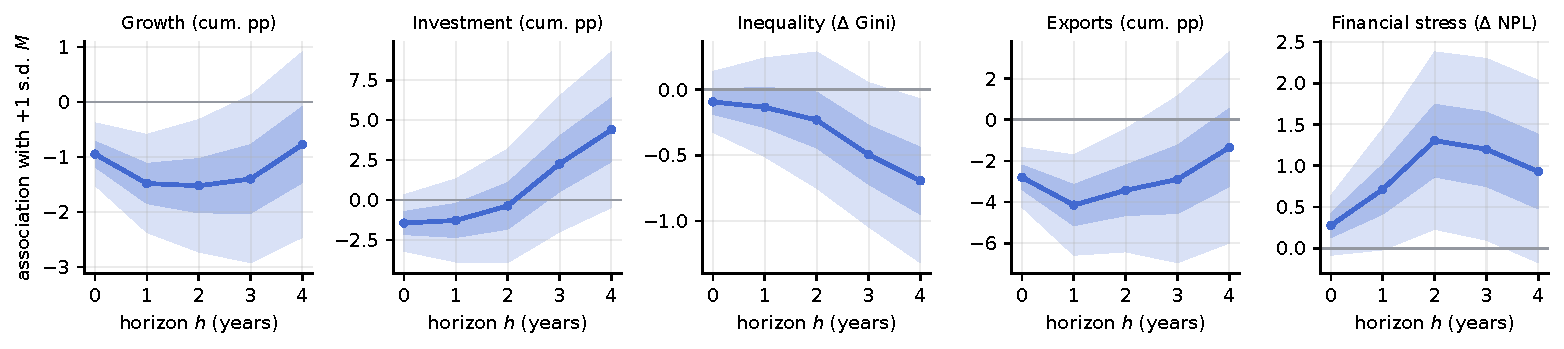
\includegraphics[width=\linewidth]{figures/fig2_lp_irfs.pdf}
\caption{Conditional mean slopes at mean conditioning states. Bands are
50 and 90 percent normal-approximation intervals from country-clustered
standard errors. Gini and NPL outcomes use observed endpoints.}\label{fig:lp}
\end{figure}
\begin{figure}[!htbp]\centering
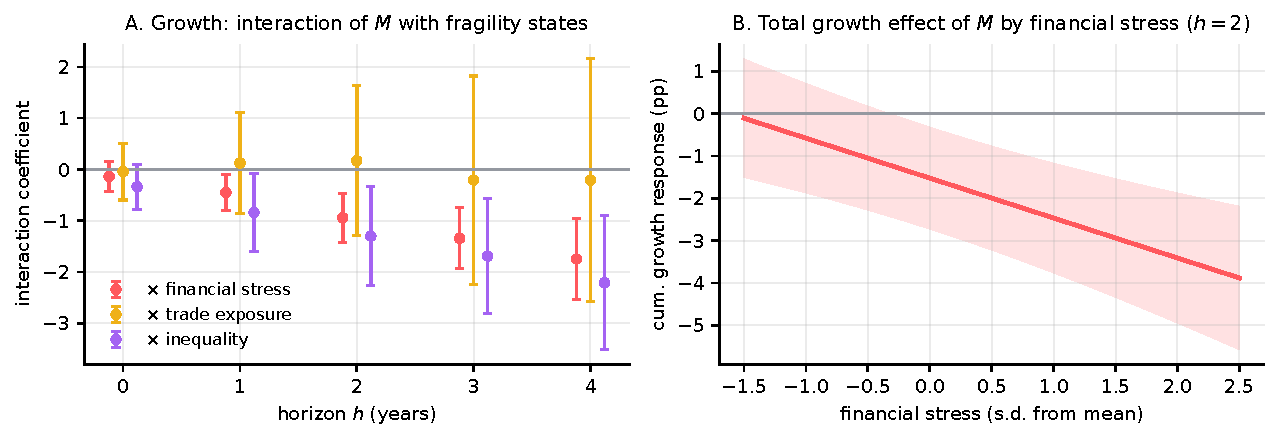
\includegraphics[width=\linewidth]{figures/fig3_amplification.pdf}
\caption{Growth interactions and the slope conditional on banking stress.
The right panel includes the estimated covariance between the index and its
stress interaction. Curves describe an estimated regression surface, not a
policy treatment response.}\label{fig:amplification}
\end{figure}

\subsection{Conditional quantiles and joint uncertainty}\label{subsec:gar}
For two-year cumulative growth, the first stage fits a two-way fixed-effects
mean regression on the index, NPLs, clipped inflation, lagged growth, log GDP
per capita and governance. Additive country and year effects are recovered
by backfitting and removed from the outcome. The second stage fits pooled
quantile regressions on the original covariates and an intercept, following
the location-shift logic of \citet{canay2011simple}. It is not quantile
regression of within-demeaned outcomes on within-demeaned regressors.

The assumption that country and year effects are common location shifts
across quantiles is substantive and cannot be justified merely because the
interest is in slopes. The procedure estimates a conditional distribution,
not the outcome that the same country would experience under a treatment.
Its covariate set is simpler than the mean-interaction specification; the
results are complementary rather than numerically identical estimands.

The revised implementation uses a linear-programming quantile solver and
\BootReps\ country-block bootstrap draws. Each draw resamples complete
country histories with replacement, assigns new identifiers to repeated
countries, and re-estimates both the mean-effect and quantile stages.
Ninety-percent percentile intervals and paired slope contrasts incorporate
the first-stage estimation step. They condition on the constructed index;
expert-coding uncertainty and residual cross-country dependence are not
fully included.
\input{tables/revised_quantiles}
\input{tables/revised_contrasts}
The point estimates at the tenth, median and ninetieth quantiles are
$\QuantileTen$, $\QuantileFifty$ and $\QuantileNinety$. Whether the lower-tail
slope is distinguishable from the center or upper tail is assessed directly
in Table~\ref{tab:contrasts}. The paired tests do not reject equal slopes (tenth versus median,
$p=0.575$; tenth versus ninetieth, $p=0.805$). All reported quantile
slope intervals include zero. The earlier claim of a statistically distinct,
roughly threefold lower-tail association is therefore withdrawn.
\begin{figure}[!htbp]\centering
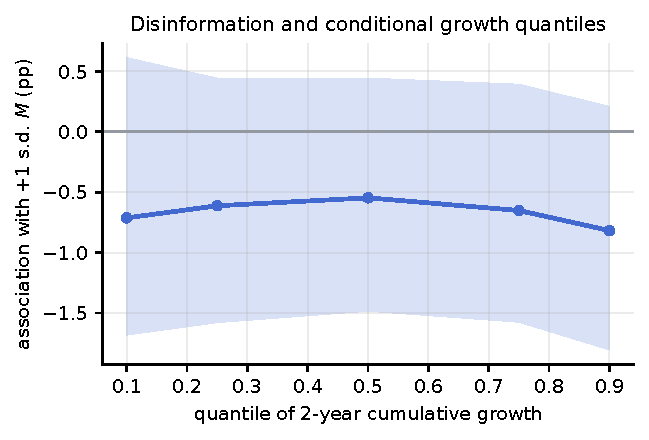
\includegraphics[width=.67\linewidth]{figures/fig4_growth_at_risk.pdf}
\caption{Conditional quantile slopes with 90 percent country-block bootstrap
intervals. Both estimation stages are refitted in each draw.}\label{fig:gar}
\end{figure}

\subsection{Reverse timing and identification limits}\label{subsec:identification}
Country and year effects remove additive persistent differences and common
year shocks. They do not remove time-varying institutional deterioration,
conflict, political instability or reverse causality. Associations with prior
outcomes are reported in Appendix~\ref{app:empirical}. Because the index is
persistent and lagged-outcome controls overlap the placebo windows, these
reverse-timing regressions are diagnostics, not experimental pre-trend tests.
In particular, controlling for a dependent variable's own overlapping lag
cannot establish the absence of confounding.

The previous draft's regional-pressure instrument interacted with internet
penetration does not establish identification. Internet exposure may affect
growth through other channels; regional pressure may reflect regional shocks;
and 2000--2004 exposure is not pre-period for a sample beginning in 2000.
Weak-IV estimates with large uncertainty cannot validate the sign. The
revised paper withdraws that evidence rather than treating it as causal
corroboration. The repository retains the original results in a clearly
marked legacy directory for audit, with the optional IV implementation
restricted to post-2004 observations and its excluded-instrument diagnostic
corrected. It is not part of the revised empirical evidence.

\subsection{Chronological forecast evaluation}\label{subsec:forecast}
At each annual origin $t=2014,\ldots,2023$, the exercise predicts GDP growth
in $t+1$ using covariates from $t-1$. Training targets end no later than
$t-1$. This conservative timing prevents use of current-year realized growth
or a future outcome in model fitting. Each model uses the same observed
sample and country intercepts; no future year effect is estimated.

The benchmark contains growth, clipped inflation, log GDP per capita, trade
openness, NPLs, private credit and government effectiveness. Missing NPL and
credit predictors can be carried forward for at most two years, never
backward. The augmented model adds the DSP index. All five component
standardizations, the rank transform, and regression scaling are fitted anew
using training observations only. Models estimate the conditional mean and
the tenth, median and ninetieth quantiles directly. The benchmark and augmented
models use identical training and evaluation samples at each origin.

\input{tables/revised_forecast}
The tenth-quantile loss gain is $\ForecastTail$ percent and the mean-squared
error gain is $\ForecastMean$ percent. Negative gains denote deterioration. None of the four loss metrics
improves at the point estimate; the tenth-quantile gain interval includes
zero. These results do not establish operational forecasting value for this
index and benchmark. Country-specific intercepts with sparse training
histories and omitted common-shock predictors may also limit performance.
Intervals resample complete target years, preserving dependence among
countries in a given year, but ten target years provide limited precision
and do not fully address serial dependence across years. The exercise is
pseudo out of sample: source vintages may contain revisions, expert scores
may be retrospective, and their actual publication calendars are not
reconstructed. A useful association in the panel therefore need not imply
an operational early-warning improvement.
